\documentclass[11pt,a4paper]{article}
\usepackage[top=2cm,bottom=2cm,left=2cm,right=2cm]{geometry}
\usepackage[T1]{fontenc}
\usepackage{newtxtext,newtxmath}
\usepackage{microtype,amsmath,booktabs,array,tabularx,graphicx,xcolor,float,caption,enumitem,tikz,tcolorbox,url}
\usepackage[colorlinks=true,linkcolor=blue!50!black,urlcolor=blue!50!black]{hyperref}
\usepackage{titlesec,fancyhdr}
\usetikzlibrary{arrows.meta,positioning}
\definecolor{navy}{HTML}{0B3D6B}
\titleformat{\section}{\Large\bfseries\color{navy}}{\thesection}{0.5em}{}
\titleformat{\subsection}{\large\bfseries\color{navy}}{\thesubsection}{0.5em}{}
\titlespacing*{\section}{0pt}{9pt}{3pt}\titlespacing*{\subsection}{0pt}{6pt}{2pt}
\setlength{\parindent}{0pt}\setlength{\parskip}{3.5pt}
\setlist{itemsep=1.5pt,topsep=2pt,parsep=0pt}
\newcolumntype{Y}{>{\raggedright\arraybackslash}X}
\pagestyle{fancy}\fancyhf{}\cfoot{\footnotesize LeakLens team guidebook \,|\, \thepage}\renewcommand{\headrulewidth}{0pt}
\captionsetup{font=small,labelfont=bf,skip=3pt}
\newtcolorbox{key}{colback=navy!6,colframe=navy!60,boxrule=0.5pt,arc=2pt,left=5pt,right=5pt,top=3pt,bottom=3pt}
\newtcolorbox{note}{colback=orange!8,colframe=orange!70!black,boxrule=0.5pt,arc=2pt,left=5pt,right=5pt,top=3pt,bottom=3pt}
\newcommand{\code}[1]{\texttt{#1}}
\renewcommand{\arraystretch}{1.08}
\begin{document}
\begin{titlepage}
\centering\vspace*{2.2cm}
{\Huge\bfseries\color{navy} LeakLens}\\[5pt]
{\LARGE Water Leak Localization System}\\[1.1cm]
{\Huge Team Guidebook}\\[0.5cm]
{\large Everything about the project in one place:\\ what it is, every formula and calculation, the dashboard terms,\\ how much was trained and tested, and what each score means}\\[1.6cm]
{\large\bfseries B.Tech Project, Semester 1}\\[2pt]
Indian Institute of Information Technology Kottayam\\[0.6cm]
\textbf{Guide:} Dr.\ Divya Sindhu Lekha\\[0.4cm]
Ashish Ranjan \,\textbullet\, Nidamanuri Kedar Vaishnav \,\textbullet\, Abhinandh Rajeev \,\textbullet\, Kadthala Hrishith Reddy\\[1.2cm]
October 2026\\[1.2cm]
\begin{minipage}{0.88\linewidth}\small
\textbf{How to use this book.} Read Part A to understand the project. Parts B to E explain how the data is made, how the system decides, and how it is trained and scored. Part F explains every word and number on the dashboard. Part G is for whoever runs the code. Every number in this book was read from the project's own result files. All data are simulated: no real sensors were used.
\end{minipage}
\end{titlepage}
\tableofcontents
\newpage

%=========================================================
\section*{Part A: Understanding the project}\addcontentsline{toc}{section}{Part A: Understanding the project}
\section{What is this project?}
Cities lose a lot of treated water through leaking pipes (the literature reports 3\% to over 50\%, depending on maintenance). A pressure drop alone does not prove a leak: a hydrant opening, a pump stopping or a tank running low also lower the pressure. So the real question is:

\begin{key}\itshape When pressure and flow change in a water network, is it a leak or a normal change, and if it is a leak, which node is it?\end{key}

\textbf{LeakLens} answers this on simulated networks. It (1) notices that something differs from a normal day, (2) names the kind of event (leak, demand change, pump or reservoir change, tank change, blocked pipe, pipe ageing, or normal), and (3) for a leak, ranks the nodes where it may be. A web dashboard shows the answer in plain language with reasons. The full project title is \emph{Water Leak Localization System}; LeakLens is its short name.

\subsection{The core idea: follow the water}
A junction behaves like a bank account: money in, money spent, money left. For water:
\[\underbrace{\text{water in}-\text{water out}}_{\text{net flow into the node}}\;=\;\underbrace{\text{water customers use}}_{\text{metered demand}}\;+\;\underbrace{\text{water that leaks}}_{\text{unmetered}}\]
If we know what customers use, then \textbf{water that leaves a node with no customer meter behind it is leaking}. We call this \emph{unaccounted flow}. A leak creates a large unaccounted flow at one node. A demand change does not (the meters record it). A pump or tank change shifts pressure over a wide area but loses no water. Almost everything in the system builds on this.

\subsection{The system in one picture}
\begin{center}
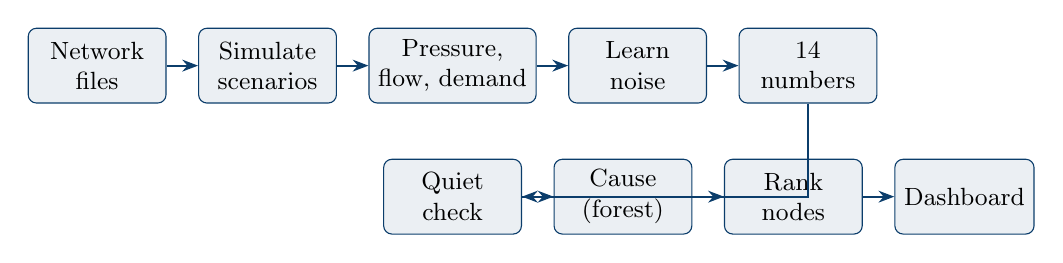
\begin{tikzpicture}[node distance=4mm,
 box/.style={draw=navy,fill=navy!8,rounded corners=3pt,minimum width=1.75cm,minimum height=0.95cm,align=center,font=\small},
 arr/.style={-{Stealth[length=2mm]},thick,navy}]
\node[box](a){Network\\files};\node[box,right=of a](b){Simulate\\scenarios};\node[box,right=of b](c){Pressure,\\flow, demand};
\node[box,right=of c](d){Learn\\noise};\node[box,right=of d](e){14\\numbers};
\node[box,below=7mm of c](f){Quiet\\check};\node[box,right=of f](g){Cause\\(forest)};\node[box,right=of g](h){Rank\\nodes};\node[box,right=of h](i){Dashboard};
\draw[arr](a)--(b);\draw[arr](b)--(c);\draw[arr](c)--(d);\draw[arr](d)--(e);\draw[arr](e.south)|-(f.east);\draw[arr](f)--(g);\draw[arr](g)--(h);\draw[arr](h)--(i);
\end{tikzpicture}\end{center}

\subsection{Headline results (test scenarios only, never seen in learning)}
\begin{center}\small\begin{tabular}{@{}lr@{}}\toprule
Question & Answer \\\midrule
Exact leak node ranked first (Top-1), 60 test leaks & \textbf{96.7\%} (58 of 60); first version 58.3\% \\
Real leak among the first five nodes (Top-5) & \textbf{98.3\%} \\
False alarms on 12 normal test days & \textbf{0.0\%} (fixed 0.5 m alarm: 41.7\%) \\
Kind of event named correctly, 139 test scenarios & \textbf{82.7\%} (on training scenarios: 95.6\%) \\
Time to analyse one scenario & about 22 ms \\\bottomrule\end{tabular}\end{center}

\section{The networks}
Three standard EPANET benchmark networks. A network is a graph: junctions joined by pipes, plus reservoirs (sources), tanks (storage) and pumps. ``Analysed'' junctions exclude unreliable nodes (Section~\ref{sec:ignored}). $\tau_P$ is the learned pressure noise threshold (Section~\ref{sec:noise}); $D_{tot}$ is the average total customer demand in L/s.
\begin{center}\small\begin{tabular}{@{}lrrrrrrrrrr@{}}\toprule
Net & Junctions & Analysed & Pipes+ & Pumps & Tanks & Reserv. & $\tau_P$ (m) & $D_{tot}$ (L/s) & Normal runs (train/test) & Ignored nodes \\\midrule
NET1 & 9 & 9 & 13 & 1 & 1 & 1 & 0.498 & 69.4 & 14/4 & none \\
NET2 & 35 & 35 & 40 & 0 & 1 & 0 & 0.535 & 20.6 & 14/4 & none \\
NET3 & 92 & 90 & 119 & 2 & 3 & 2 & 0.582 & 690.7 & 14/4 & 601, 61 \\
\bottomrule\end{tabular}\end{center}
Net2 has no reservoir or pump; one junction with negative demand acts as its supply. (Pipes+ counts all links including pumps.)

%=========================================================
\section*{Part B: The data}\addcontentsline{toc}{section}{Part B: The data}
\section{Scenarios}
A \textbf{scenario} is one 24-hour simulation of a network in which one thing (or a few together) differs from a normal day. The \textbf{baseline} is the normal day. For every scenario we save, once per hour: pressure at every node, flow in every pipe, and the demand actually delivered at every node (what a customer meter reads; leak flow is not included). We also save the \emph{true answer} (kind of event, leak node) to score the system; it is never given to the model as input.
\begin{center}\small\begin{tabularx}{\linewidth}{@{}>{\bfseries}p{2.1cm}p{0.8cm}Y@{}}\toprule
Kind & Count & Parameters used \\\midrule
Leak & 299 & hole at one junction; areas 0.0001 / 0.0003 / 0.001 / 0.003 / 0.01 m$^2$ (tiny / small / medium / large / burst); start 12:00 (also 2, 8, 20); every junction in each network; noisy copies; \emph{hidden behind} a global demand $\times1.3$, a hydrant, a closed pipe or a pump outage \\
Demand change & 60 & one node $\times1.5$ or $\times0.5$ from 12:00; all nodes $\times1.3$ or $\times0.7$; hydrant 0.01 m$^3$/s for 10:00--14:00 \\
Pump / reservoir & 54 & pump off for 2, 4 or 6 h while it normally runs; reservoir head $\pm2,\pm5,\pm10$ m from 12:00 \\
Tank change & 60 & tank starts at 10, 20, 30, 70 or 90\% full; or its pipe is closed at 10:00 \\
Blocked pipe & 48 & a busy pipe closed from 10:00, or throttled (minor loss 5000) \\
Pipe ageing & 42 & every pipe's Hazen--Williams $C$ multiplied by 0.6--0.95 \\
Normal day & 54 & no change; sensor noise only (16 noisy, 1 very light, 1 clean per network) \\\bottomrule\end{tabularx}\end{center}
Most non-leak scenarios also have a ``noisy'' twin. A leak scenario count includes the hidden-behind variants.

\subsection{What each event does (the physics)}
\begin{itemize}
\item \textbf{Leak.} Water leaves through a hole: $Q_\ell(t)=C_d\,A\,\sqrt{2\,g\,P(t)}$ with $C_d=0.75$, hole area $A$, $g=9.81$ m/s$^2$, pressure head $P$ at the node. More pressure means more loss. Flow towards the node rises; pressure falls around it, most at the node. \emph{Local and unmetered.}
\item \textbf{Demand change.} Customer use at node $i$: $D_i(t)=D_{\text{base},i}\,m(t)\,f$, where $m(t)$ is the daily pattern and $f$ the factor. Pressure falls where use is heavy, like a leak, but the extra flow is \emph{metered}.
\item \textbf{Pump outage / reservoir head.} Boundary conditions change: a pump off removes its added head so pressure falls over its whole area and tanks start to supply; a reservoir shifted by $\Delta h$ shifts pressure everywhere by about $\Delta h$. No water is lost.
\item \textbf{Tank level / isolation.} Different starting level changes the head the tank supplies; closing its pipe stops all flow through it. No water is lost.
\item \textbf{Blocked pipe.} Closed pipe: flow reroutes, pressure falls downstream and may rise upstream. No water is lost.
\item \textbf{Ageing.} Head loss $h_f=\dfrac{10.67\,L\,Q^{1.852}}{C^{1.852}\,d^{4.87}}$ grows as the roughness coefficient $C$ falls: wide, smooth pressure loss, largest where flow is highest. No water is lost.
\end{itemize}

\subsection{Sensor noise}
Gaussian errors with fixed seeds are added to saved readings of ``noisy'' scenarios: \emph{low} $=0.05$ m on pressure and 0.5\% on flows and demands; \emph{high} $=0.2$ m and 2\%. The baseline stays clean: it is the model's expectation. Simulation uses pressure-dependent demand (the engine reduces delivered demand when pressure is low).

\begin{figure}[H]\centering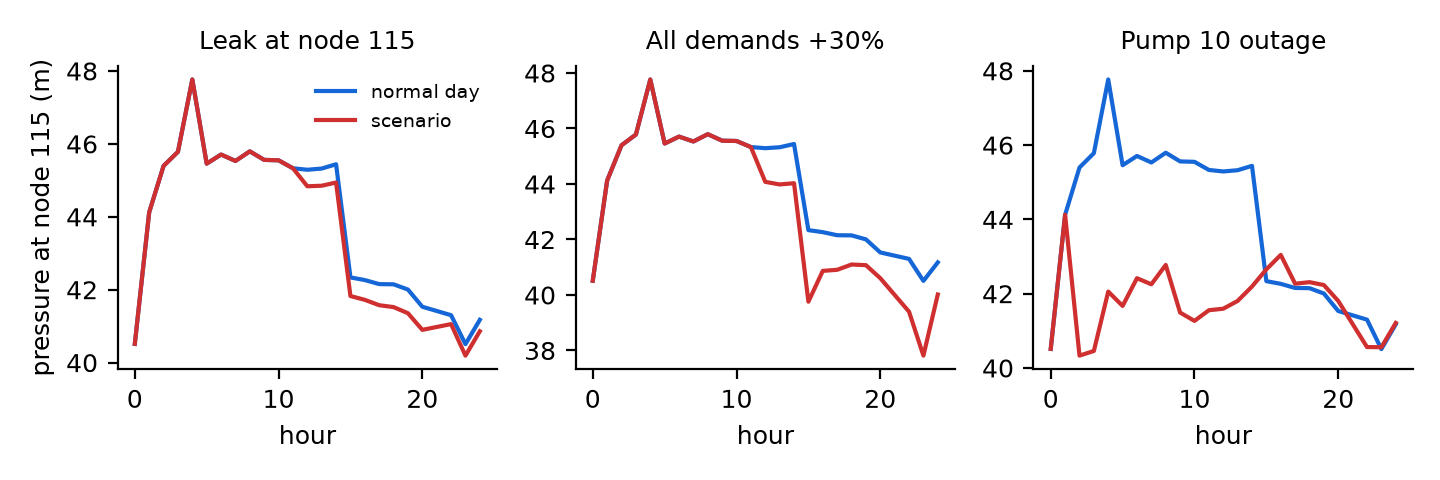
\includegraphics[width=0.95\linewidth]{figures/fig_pressure.png}\caption{Pressure at one Net3 node on a normal day (blue) and in a leak, a demand surge and a pump outage (red).}\end{figure}

\subsection{Unreliable nodes and hours}\label{sec:ignored}
A 1\% demand probe is run on each network. Nodes whose pressure swings more than 5 m, and hours where 90\% of nodes swing more than 0.5 m, are called ill-conditioned (pump-switching artefacts) and are ignored in all analysis: Net3 nodes \textbf{61} and \textbf{601} and hour \textbf{21:00}. Scenarios whose hydraulics did not converge were dropped (three Net3 blockage candidates).

%=========================================================
\section*{Part C: How much was trained and how much tested}\addcontentsline{toc}{section}{Part C: Trained vs tested}
\section{The 80/20 split}
\begin{key}Testing on scenarios the system learned from would look perfect and prove nothing. So some scenarios are kept completely aside.\end{key}
All \textbf{617} scenarios were split once (random seed 42, \code{ml\_pipeline/split.py}) into \textbf{478 for learning (training, about 80\%)} and \textbf{139 for testing (about 20\%)}.
\begin{center}\small\begin{tabular}{@{}lrrr@{}}\toprule
Kind of event & All & Train & Test \\\midrule
Normal day & 54 & 42 & 12 \\
Leak & 299 & 232 & 67 \\
Demand change & 60 & 48 & 12 \\
Pump / reservoir & 54 & 42 & 12 \\
Tank change & 60 & 48 & 12 \\
Blocked pipe & 48 & 36 & 12 \\
Pipe ageing & 42 & 30 & 12 \\
\midrule
Total & 617 & 478 & 139 \\
\bottomrule\end{tabular}\end{center}
Per network, train/test counts by kind (N = normal, L = leak, D = demand, S = pump/reservoir, T = tank, B = blocked, A = ageing; Net2 has no pump or reservoir events):
\begin{center}\small\begin{tabular}{@{}lrrrrrrrrrr@{}}\toprule
Net & All & Train & Test & N & L & D & S & T & B & A \\\midrule
NET1 & 155 & 122 & 33 & 14/4 & 46/11 & 16/4 & 14/4 & 10/2 & 12/4 & 10/4 \\
NET2 & 171 & 127 & 44 & 14/4 & 65/26 & 16/4 & 0/0 & 10/2 & 12/4 & 10/4 \\
NET3 & 291 & 229 & 62 & 14/4 & 121/30 & 16/4 & 28/8 & 28/8 & 12/4 & 10/4 \\
\bottomrule\end{tabular}\end{center}
\textbf{Rules of the split.}
\begin{itemize}
\item \textbf{What learns from the training scenarios only:} (1) the noise thresholds (from the training normal runs, 14 per network); (2) the random forest and the decision tree.
\item \textbf{What is not learned:} the leak-ranking formula (a fixed formula) and the quiet check. Their settings (weight 0.3, cut-offs) were chosen during development while looking at all scenarios, before the split, and not re-tuned afterwards.
\item \textbf{What is measured on the test scenarios only:} every accuracy, precision, recall, F1, false-alarm, Top-$k$, hop and timing figure in this book. Training-set figures are shown only to expose over-fitting.
\item \textbf{Near-copies stay together.} All leaks at the same junction (every size, start time, noise level, hidden-behind variant) go to the same side; a scenario and its noisy twin go to the same side. Otherwise a test scenario could be almost identical to a training one.
\item \textbf{Stratified.} Each network and each kind of event is split about 80/20, so the test set has 12 of every non-leak kind and 60+ leaks (some leaks sit on ignored nodes and are not scored).
\item The dashboard tags every scenario \emph{Unseen test} or \emph{Training}.
\end{itemize}
\begin{note}\textbf{Caution.} The test set is small (139 scenarios; 60 scored leaks; 12 normal days). One missed leak moves Top-1 by $1/60\approx1.7$ points, and the split was made once, so every percentage has a wide margin of error.\end{note}

%=========================================================
\section*{Part D: How the system decides}\addcontentsline{toc}{section}{Part D: How the system decides}
\section{Step-by-step with formulas}
Notation: $P^0_i(t)$ and $P^1_i(t)$ are pressures at node $i$, hour $t$, on the normal day and in the scenario; $Q^0_p,Q^1_p$ pipe flows; $D^0_i,D^1_i$ metered demands. Set $\mathcal I$ is the analysed junctions.

\subsection{Step 1: pressure drop with persistence}
Residual $r_i(t)=P^0_i(t)-P^1_i(t)$. To ignore one-off errors, a drop counts only if it holds for two consecutive hours:
\[\text{persistent peak}(x_i)=\max_t\ \min\{x_i(t),\,x_i(t{+}1)\}.\]
The drop of node $i$ in noise units is $d_i=\max\{0,\text{peak}(r_i)\}/\tau_P$; the rise is $g_i=\max\{0,\text{peak}(-r_i)\}/\tau_P$.

\subsection{Step 2: learn the noise}\label{sec:noise}
From the 14 training normal runs of each network: $\tau_P=\max\{0.1\,\text{m},\;4\,\sigma_P\}$ where $\sigma_P$ is the standard deviation of all pressure residuals over analysed nodes and hours. In the same way: $\sigma_{f,p}$ (per pipe flow), $\sigma_{D,i}$ (per node demand) and $\sigma_{a,i}$ (per node unaccounted flow, Step 3). $D_{tot}$ is the mean over time of the total positive baseline demand. A value of ``1'' in noise units means \emph{exactly at the noise limit}.

\subsection{Step 3: unaccounted flow}
Net inflow to node $i$ is $\text{div}_i(t)=\sum_p \operatorname{sign}(p,i)\,Q_p(t)$, where $\operatorname{sign}=+1$ if pipe $p$ ends at $i$ and $-1$ if it starts there. Mass balance: $\text{div}_i=D_i+Q_{\ell,i}$. So the leak flow is
\[a_i(t)=\big[\text{div}^1_i(t)-\text{div}^0_i(t)\big]-\big[D^1_i(t)-D^0_i(t)\big]=Q_{\ell,i}(t).\]
Its persistent peak in noise units: $\;a_i=\max\{0,\text{peak}(a_i(t))\}\,/\,(4\,\sigma_{a,i})$. In noise-free data it equals the leak flow at the leak node and 0 elsewhere. When demand meters are unavailable the second bracket is dropped.

\begin{figure}[H]\centering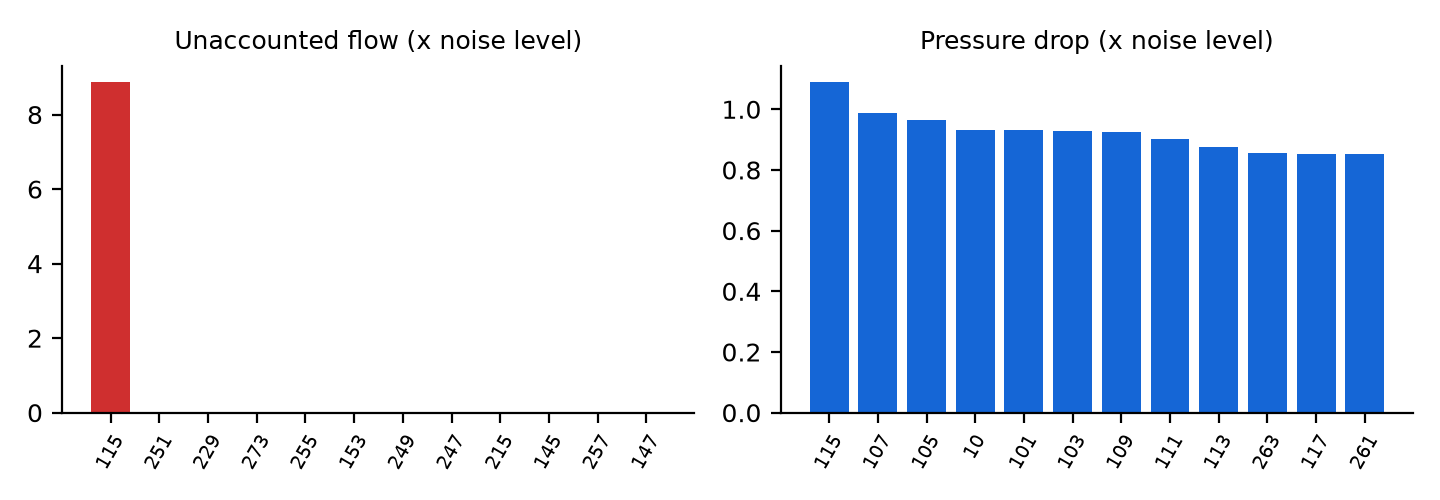
\includegraphics[width=0.95\linewidth]{figures/fig_signals.png}\caption{A leak at one Net3 node: unaccounted flow (left) is large only at the leak node; pressure drop (right) is also high at its neighbours.}\end{figure}

\subsection{Step 4: fourteen numbers}
Medians over all scenarios of that kind (from \code{features.csv}); see Section~\ref{sec:examples} for individual scenarios. $z_p=\text{peak}|Q^1_p-Q^0_p|/(4\sigma_{f,p})$; $\Delta S(t)$ is the change in total reservoir supply and $\Delta T(t)$ the change in net tank flow; $k$ runs over pumps; $z^D_i=\text{peak}|\Delta D_i|/(4\sigma_{D,i})$.
\begin{center}\footnotesize\begin{tabularx}{\linewidth}{@{}>{\ttfamily}p{2.45cm}p{3.5cm}p{3.0cm}rrrrr@{}}\toprule
Name & Meaning & Formula & Normal & Leak & Demand & Pump/res. & Blocked \\\midrule
\texttt{drop\_ratio} & Largest pressure drop in noise units & $\max_i d_i$ & 0.20 & 4.25 & 1.11 & 2.61 & 6.82 \\
\texttt{frac\_hit} & Share of junctions with a drop above noise & mean$(d_i>1)$ & 0.00 & 0.56 & 0.03 & 0.01 & 0.44 \\
\texttt{median\_ratio} & Typical (median) drop & median$_i\,d_i$ & 0.09 & 1.18 & 0.14 & 0.35 & 0.36 \\
\texttt{conc\_drop} & Drop concentrated at one node & $\max d_i/(\sum d_i)$ & 0.05 & 0.05 & 0.07 & 0.12 & 0.09 \\
\texttt{rise\_ratio} & Largest pressure rise & $\max_i g_i$ & 0.20 & 0.54 & 0.44 & 2.62 & 3.29 \\
\texttt{frac\_rise} & Share of junctions with a rise & mean$(g_i>1)$ & 0.00 & 0.00 & 0.00 & 0.02 & 0.15 \\
\texttt{flow\_frac} & Share of pipes with changed flow & mean$(z_p>1)$ & 0.00 & 0.60 & 0.35 & 0.47 & 0.65 \\
\texttt{source\_change} & Reservoir supply change / demand & $\max_t|\Delta S(t)|/D_{tot}$ & 0.01 & 0.01 & 0.01 & 0.37 & 0.01 \\
\texttt{tank\_change} & Tank net-flow change / demand & $\max_t|\Delta T(t)|/D_{tot}$ & 0.01 & 0.43 & 0.23 & 0.37 & 0.01 \\
\texttt{pump\_drop} & Pump flow lost (1 = off) & $\max (Q^0_k-Q^1_k)/\max Q^0_k$ & 0.01 & 0.00 & 0.00 & 0.09 & 0.01 \\
\texttt{unacc\_ratio} & Largest unaccounted flow in noise units & $\max_i a_i$ & 0.25 & 11.16 & 0.06 & 0.08 & 0.07 \\
\texttt{unacc\_conc} & Unaccounted flow concentrated at one node & $\max a_i/\sum a_i$ & 0.07 & 1.00 & 0.02 & 0.01 & 0.02 \\
\texttt{demand\_frac} & Share of nodes with metered-demand change & mean$(z^D_i>1)$ & 0.00 & 0.00 & 0.03 & 0.00 & 0.00 \\
\texttt{demand\_total} & Signed total demand change / demand & $\sum_i\Delta D_i/D_{tot}$ & -0.00 & -0.00 & 0.01 & -0.00 & -0.00 \\
\bottomrule\end{tabularx}\end{center}

\subsection{Step 5: the quiet check}
If $\text{drop\_ratio}<1$, $\text{rise\_ratio}<1$, $\text{unacc\_ratio}<1$, $\text{flow\_frac}<0.1$ and $\text{demand\_frac}=0$, everything is within noise: the answer is \textbf{normal day} and nothing else runs. This is why normal days give no false alarms (and why leaks inside the noise cannot be seen).

\subsection{Step 6: which kind of event?}
A \textbf{random forest} (scikit-learn; 300 decision trees; each tree votes; balanced class weights so rare kinds are not ignored; seed 0; no tuning) maps the 14 numbers to a probability for each of 7 kinds. Highest probability = verdict. Confidence label: \textbf{High} $\ge85\%$, \textbf{Medium} $\ge60\%$, else \textbf{Low}. A depth-4 decision tree is trained too (rules in \code{decision\_rules.txt}) for readability; it is less accurate and not used for the verdict. Training uses the 478 training rows only.

\subsection{Step 7: rank the nodes (only if the verdict is leak)}
For each junction, with $A_i=a_i/\max_j a_j$ (set to 0 for all nodes if $\max_j a_j<1$) and $D_i=d_i/\max_j d_j$:
\[\textbf{score}_i=A_i+0.3\,D_i.\]
Sort descending. First node = \textbf{Top-1}. Neighbour smoothing ($+\beta\cdot$ mean score of adjacent nodes, $\beta=0.3$) was tested and is \emph{off} (no gain). Error of a guess: \textbf{hops} = pipes on the shortest path to the true node; \textbf{metres} = pipe length on that path (pumps and valves count as 1 m). \textbf{Search region} = the first node plus its direct neighbours.

\subsection{Worked example: leak at node 15 (net3\_leak\_15, a test scenario)}\label{sec:example}
Network Net3, hole area 0.001 m$^2$ from 12:00. $\tau_P=0.582$ m.
\begin{center}\small\begin{tabular}{@{}cccc@{}}\toprule
Hour & Normal $P^0$ (m) & Scenario $P^1$ (m) & Residual $r$ (m) \\\midrule
10:00 & 39.74 & 39.74 & 0.00 \\
11:00 & 35.98 & 35.98 & 0.00 \\
12:00 & 35.91 & 29.22 & 6.69 \\
13:00 & 35.88 & 29.20 & 6.68 \\
14:00 & 35.91 & 29.23 & 6.68 \\
15:00 & 35.44 & 28.81 & 6.63 \\
16:00 & 38.77 & 35.92 & 2.85 \\
\bottomrule\end{tabular}\end{center}
\begin{itemize}
\item \textbf{Step 1:} the residual stays at about 6.68 m for several hours from 12:00; persistent peak $=6.68$ m; $d=6.68/0.582=11.49$ noise units.
\item \textbf{Step 3:} unaccounted flow peak $=0.01987$ m$^3$/s ($=19.9$ L/s). Node noise $\sigma_a=0.000497$, so $4\sigma_a=0.001988$ and $a=0.01987/0.001988=9.99$ noise units (about ten times the noise).
\item \textbf{Step 6:} the model gives Leak 94\%, Normal day 2\%, Blocked pipe 2\%: verdict \emph{leak}.
\item \textbf{Step 7:} the largest $a$ and $d$ in the network are both at node 15, so $A=D=1$:
\end{itemize}
\begin{center}\small\begin{tabular}{@{}cccccc@{}}\toprule
Rank & Node & $A$ & $D$ & Score & Hops from truth \\\midrule
1 & 15 & 1.00 & 1.00 & 1.00+0.3$\times$1.00 = 1.30 & 0 \\
2 & 143 & 0.00 & 0.60 & 0.00+0.3$\times$0.60 = 0.18 & 1 \\
3 & 141 & 0.00 & 0.25 & 0.00+0.3$\times$0.25 = 0.08 & 2 \\
4 & 145 & 0.00 & 0.21 & 0.00+0.3$\times$0.21 = 0.06 & 3 \\
\bottomrule\end{tabular}\end{center}
The true node is first (0 hops): a \textbf{Top-1 success}. Its neighbours have almost no unaccounted flow ($A\approx0$) but a big pressure drop, so they only score about $0.3D$.

\subsection{Fingerprints of the other kinds (Net3 test scenarios)}\label{sec:examples}
\begin{center}\footnotesize\begin{tabular}{@{}lrrrrrr@{}}\toprule
 & Leak & Demand change & Pump outage & Tank change & Blocked pipe & Ageing \\\midrule
\texttt{drop\_ratio} & 11.49 & 0.03 & 50.59 & 5.71 & 13.33 & 29.96 \\
\texttt{frac\_hit} & 0.08 & 0.00 & 0.99 & 0.31 & 0.62 & 1.00 \\
\texttt{rise\_ratio} & 0.17 & 4.41 & 3.42 & 0.14 & 64.39 & 7.30 \\
\texttt{flow\_frac} & 0.30 & 0.12 & 0.84 & 0.34 & 0.87 & 0.87 \\
\texttt{source\_change} & 0.01 & 0.00 & 0.47 & 0.00 & 0.49 & 0.47 \\
\texttt{tank\_change} & 0.03 & 0.02 & 0.47 & 0.00 & 0.49 & 0.47 \\
\texttt{pump\_drop} & 0.00 & 0.00 & 1.00 & 0.00 & 0.43 & 0.32 \\
\texttt{unacc\_ratio} & 9.99 & 0.00 & 0.00 & 0.00 & 0.00 & 0.00 \\
\texttt{demand\_frac} & 0.00 & 0.01 & 0.00 & 0.00 & 0.00 & 0.00 \\
\midrule
Verdict (confidence) & Leak (94\%) & Demand change (59\%) & Pump / reservoir (97\%) & Tank change (84\%) & Blocked pipe (90\%) & Pump / reservoir (35\%) \\\bottomrule\end{tabular}\end{center}
Read across: only the leak has a large \code{unacc\_ratio}; the demand change is metered (\code{demand\_frac}) with no unaccounted flow; the pump outage shows \code{pump\_drop} $=1$ and large supply/tank change; the throttled pipe shows a large pressure \emph{rise} (\code{rise\_ratio}) next to drops. The ageing example is a wrong answer: it is called a pump/reservoir change with only 35\% confidence, because ageing and a pump event both lower pressure widely without losing water.

%=========================================================
\section*{Part E: Metrics and scores}\addcontentsline{toc}{section}{Part E: Metrics and scores}
\section{What each metric means and how it is calculated}
\subsection{Detection: is something wrong?}
A scenario is \emph{positive} if any abnormal event happened and \emph{negative} if it is a normal day. Counts: TP (real problem, system says problem), FN (real problem, system says normal: a miss), FP (normal day, system says problem: a false alarm), TN (normal day, system says normal).
\[\text{precision}=\frac{TP}{TP+FP},\quad \text{recall}=\frac{TP}{TP+FN},\quad F_1=\frac{2\,\text{precision}\cdot\text{recall}}{\text{precision}+\text{recall}},\quad \text{false-alarm rate}=\frac{FP}{FP+TN}.\]
Three detectors compared (\textbf{fixed 0.5 m}: any node's drop above 0.5 m at any hour; \textbf{learned}: persistent drop above $\tau_P$ at an analysed node; \textbf{full system}: verdict is not ``normal day''). Test scenarios: 139 (12 normal).
\begin{center}\small\begin{tabular}{@{}lccccrrrr@{}}\toprule
Detector & Precision & Recall & $F_1$ & False alarm & TP & FP & FN & TN \\\midrule
Fixed 0.5 m alarm & 95.7\% & 87.4\% & 91.4\% & 41.7\% & 111 & 5 & 16 & 7 \\
Learned pressure threshold & 100.0\% & 77.2\% & 87.1\% & 0.0\% & 98 & 0 & 29 & 12 \\
Full system & 100.0\% & 93.7\% & 96.7\% & 0.0\% & 119 & 0 & 8 & 12 \\
\bottomrule\end{tabular}\end{center}
\textit{Calculation (full system):} precision $=119/(119+0)=$ 100.0\%; recall $=119/(119+8)=$ 93.7\%; $F_1=$ 96.7\%; false-alarm rate $=0/(0+12)=$ 0.0\%. A fixed 0.5 m alarm fires on normal noise, hence 41.7\%.

\subsection{Classification: which kind of event?}
Confusion matrix on the 139 test scenarios (rows = truth, columns = system; a dot is 0):
\begin{center}\small\begin{tabular}{@{}lrrrrrrrr@{}}\toprule
Truth $\backslash$ system & Normal & Leak & Demand & Pump & Tank & Blocked & Ageing & Total \\\midrule
Normal day & 12 & . & . & . & . & . & . & 12 \\
Leak & 6 & 60 & . & . & 1 & . & . & 67 \\
Demand change & . & . & 12 & . & . & . & . & 12 \\
Pump / reservoir & 2 & . & . & 8 & 2 & . & . & 12 \\
Tank change & . & . & . & . & 8 & . & 4 & 12 \\
Blocked pipe & . & 1 & . & . & 1 & 9 & 1 & 12 \\
Pipe ageing & . & . & . & 4 & 2 & . & 6 & 12 \\
\bottomrule\end{tabular}\end{center}
\textbf{Accuracy} $=$ diagonal $/$ total $=115/139=$ \textbf{82.7\%}. On the 478 training scenarios accuracy is 95.6\% (the gap shows partial memorising). Per kind, with TP = diagonal, FP = column total $-$ TP, FN = row total $-$ TP:
\begin{center}\footnotesize\begin{tabular}{@{}lrrrccc@{}}\toprule
Kind & TP & FP & FN & Precision & Recall & $F_1$ \\\midrule
Normal day & 12 & 8 & 0 & 12/(12+8) = 60.0\% & 12/(12+0) = 100.0\% & 75.0\% \\
Leak & 60 & 1 & 7 & 60/(60+1) = 98.4\% & 60/(60+7) = 89.6\% & 93.8\% \\
Demand change & 12 & 0 & 0 & 12/(12+0) = 100.0\% & 12/(12+0) = 100.0\% & 100.0\% \\
Pump / reservoir & 8 & 4 & 4 & 8/(8+4) = 66.7\% & 8/(8+4) = 66.7\% & 66.7\% \\
Tank change & 8 & 6 & 4 & 8/(8+6) = 57.1\% & 8/(8+4) = 66.7\% & 61.5\% \\
Blocked pipe & 9 & 0 & 3 & 9/(9+0) = 100.0\% & 9/(9+3) = 75.0\% & 85.7\% \\
Pipe ageing & 6 & 5 & 6 & 6/(6+5) = 54.5\% & 6/(6+6) = 50.0\% & 52.2\% \\
\bottomrule\end{tabular}\end{center}
\begin{figure}[H]\centering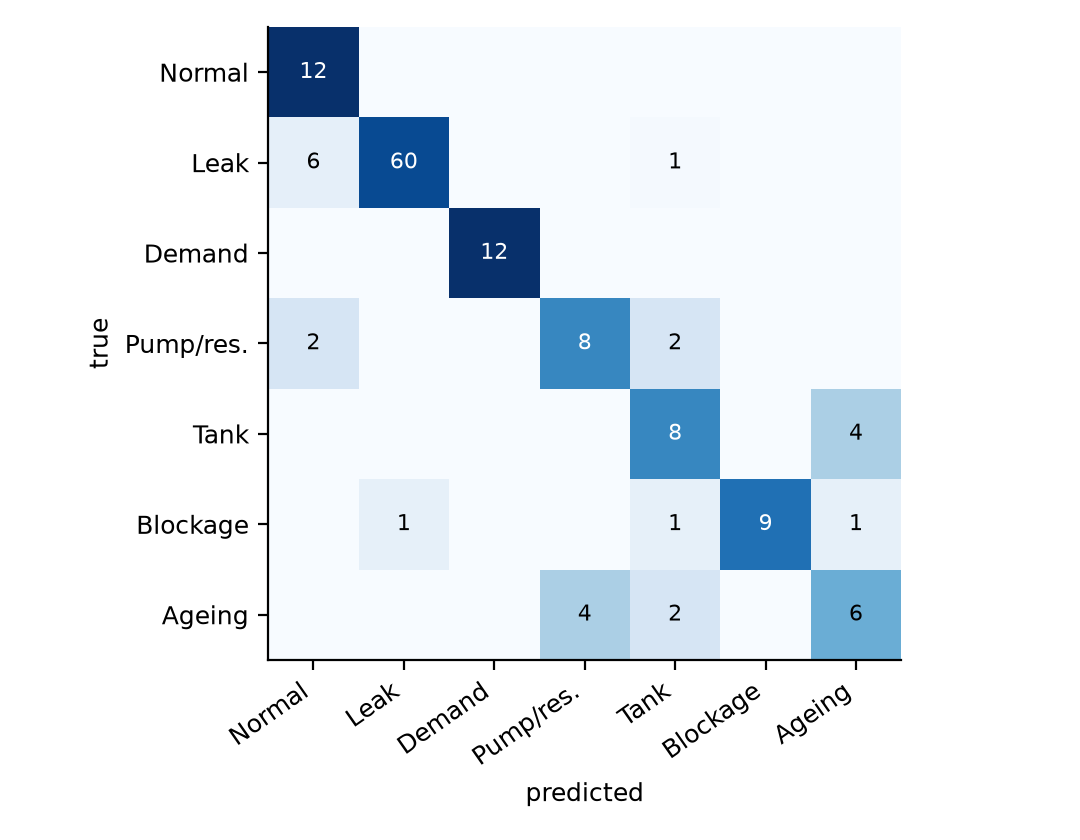
\includegraphics[width=0.52\linewidth]{figures/fig_confusion.png}\caption{The confusion matrix as a picture (darker = more scenarios).}\end{figure}
\textbf{Macro-F1} = plain average of the seven $F_1$ values $=$ \textbf{76.4\%} (each kind counts equally, so weak small kinds pull it down). Of the leaks, 89.6\% were named leaks; the 7 that were not are all at Net3 node 601, an ignored pump-outage node, and only 1.4\% of non-leaks were wrongly called a leak.

\subsection{Localization: where is the leak?}
\textbf{Rank} $r_s$ = position of the true node in the sorted list. \textbf{Top-$k$} $=\frac1N\sum_s\mathbf 1[r_s\le k]$. \textbf{Mean hops} $=\frac1N\sum_s\text{hops}(\hat n_s,n_s)$. \textbf{Within 1 hop} = share with hops $\le1$. \textbf{End-to-end} = share where the verdict is leak \emph{and} $r_s=1$. \textbf{Time} = mean seconds for ranking one scenario.
\begin{center}\small\begin{tabular}{@{}lcccccc@{}}\toprule
Method (60 test leaks) & Top-1 & Top-3 & Top-5 & Mean hops & $\le$1 hop & Mean metres \\\midrule
First version & 58.3\% & 70.0\% & 71.7\% & 3.35 & 58.3\% & 1774 \\
\textbf{Final method} & 96.7\% & 98.3\% & 98.3\% & 0.13 & 96.7\% & 60 \\
Final + smoothing & 96.7\% & 98.3\% & 98.3\% & 0.13 & 96.7\% & 60 \\
Final, no demand meters & 93.3\% & 98.3\% & 98.3\% & 0.72 & 93.3\% & 303 \\
Pressure only & 60.0\% & 70.0\% & 70.0\% & 3.05 & 61.7\% & 1208 \\
Pressure only + smoothing & 50.0\% & 63.3\% & 65.0\% & 3.18 & 58.3\% & 1244 \\
\bottomrule\end{tabular}\end{center}
\textit{Calculation:} Top-1 $=58/60=$ 96.7\% (first version $35/60=$ 58.3\%). End-to-end 96.7\%. Time about 22 ms. On the 231 training leaks the final method scores 97.8\% (almost the same, because the ranking is a formula, not trained).\\
\begin{figure}[H]\centering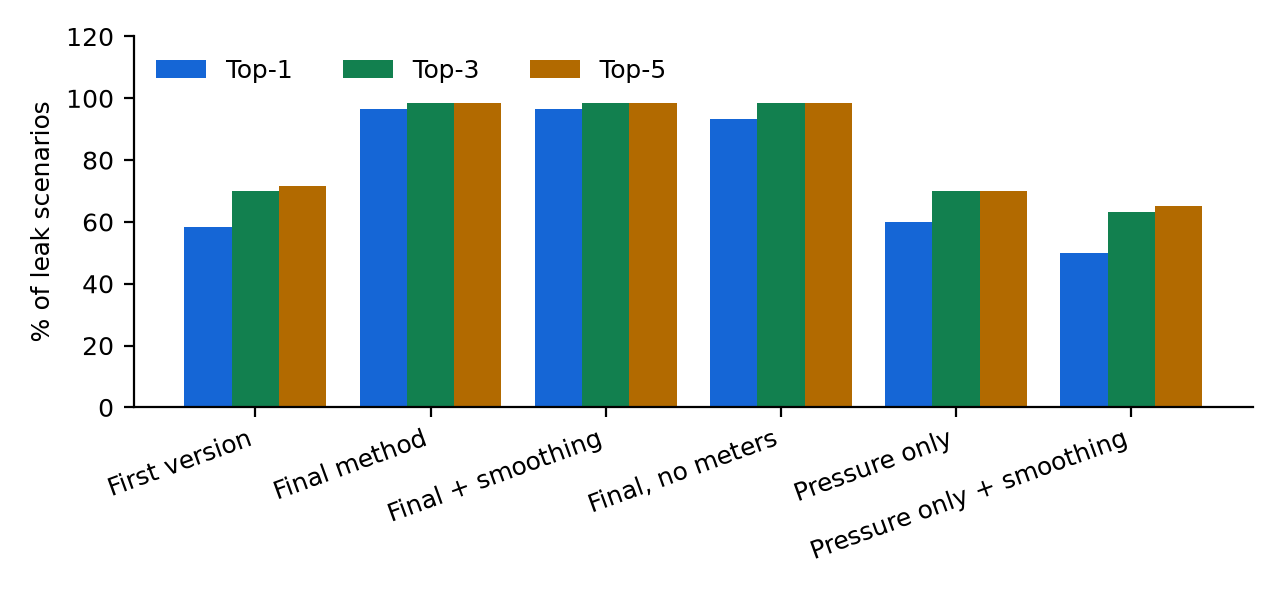
\includegraphics[width=0.72\linewidth]{figures/fig_localization.png}\caption{Top-1, Top-3 and Top-5 of each localization method on the test leaks.}\end{figure}
\textit{What the variants show:} unaccounted flow lifts Top-1 from 58.3\% to 96.7\%; without demand meters 93.3\%; pressure alone 60.0\%; neighbour smoothing 96.7\% (no help).

\subsection{By leak type, node type and network (final method, test leaks)}
\begin{center}\small\begin{tabular}{@{}lcccc@{}}\toprule
Group & Leaks & Top-1 & Top-5 & Mean hops \\\midrule
Hidden behind another event & 10 & 100.0\% & 100.0\% & 0.00 \\
With sensor noise & 4 & 100.0\% & 100.0\% & 0.00 \\
Size variations & 20 & 90.0\% & 95.0\% & 0.40 \\
Start-time variations & 4 & 100.0\% & 100.0\% & 0.00 \\
Leak at a junction & 22 & 100.0\% & 100.0\% & 0.00 \\
\midrule
Dead End & 17 & 100.0\% & 100.0\% & 0.00 \\
Hub & 1 & 100.0\% & 100.0\% & 0.00 \\
Inline & 42 & 95.2\% & 97.6\% & 0.19 \\
NET1 & 11 & 100.0\% & 100.0\% & 0.00 \\
NET2 & 26 & 92.3\% & 96.2\% & 0.31 \\
NET3 & 23 & 100.0\% & 100.0\% & 0.00 \\
\bottomrule\end{tabular}\end{center}
\subsection{By leak size}
\begin{center}\small\begin{tabular}{@{}cccccc@{}}\toprule
Area (m$^2$) & Test leaks & Noticed by pressure & Called a leak & Top-1 & Top-5 \\\midrule
0.0001 & 4 & 75.0\% & 100.0\% & 100.0\% & 100.0\% \\
0.0003 & 4 & 100.0\% & 100.0\% & 100.0\% & 100.0\% \\
0.001 & 4 & 100.0\% & 100.0\% & 100.0\% & 100.0\% \\
0.003 & 4 & 100.0\% & 100.0\% & 100.0\% & 100.0\% \\
0.01 & 4 & 100.0\% & 100.0\% & 50.0\% & 75.0\% \\
\bottomrule\end{tabular}\end{center}
\begin{figure}[H]\centering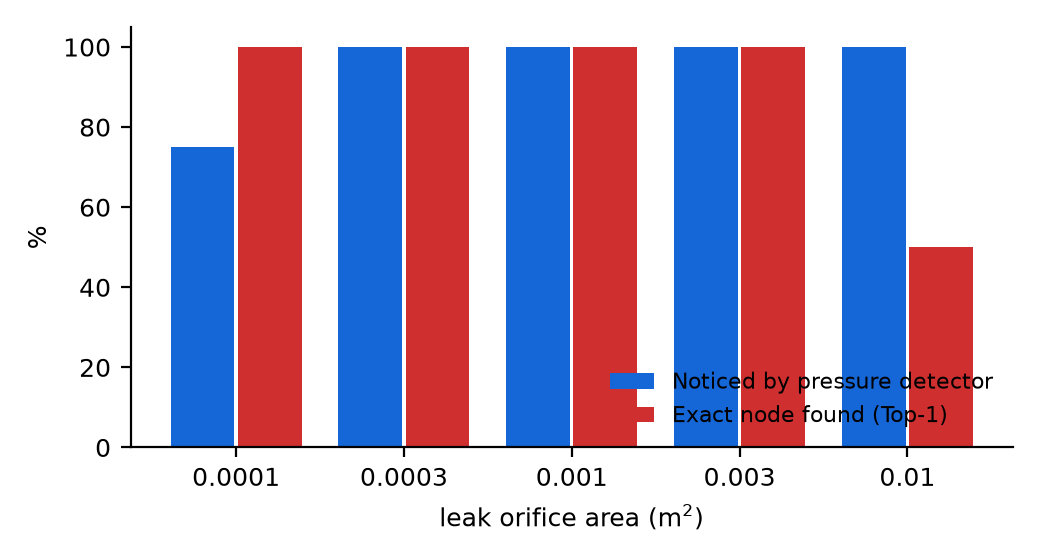
\includegraphics[width=0.55\linewidth]{figures/fig_size.png}\caption{Detection and exact-node success by leak size.}\end{figure}
Only four test leaks per size, so read loosely. The biggest leak collapses pressure across the whole network, so its exact node is the hardest to pick.

\subsection{Unseen network (leave-one-network-out)}
Train on the training scenarios of two networks, test on the third network's test scenarios:
\begin{center}\small\begin{tabular}{@{}lccccc@{}}\toprule
Unseen network & Test scen. & Accuracy & Leak recall & Leak precision & Accuracy, no meters \\\midrule
NET1 & 33 & 48.5\% & 100.0\% & 100.0\% & 45.5\% \\
NET2 & 44 & 81.8\% & 92.3\% & 100.0\% & 75.0\% \\
NET3 & 62 & 54.8\% & 73.3\% & 100.0\% & 14.5\% \\
\bottomrule\end{tabular}\end{center}
Leaks carry over; telling pump, tank, blockage and ageing apart does not yet. Without per-node demand meters (all networks pooled) accuracy falls to 74.1\%, and to 14.5\% on an unseen Net3. This is the main Semester~2 item.

%=========================================================
\section*{Part F: The dashboard, term by term}\addcontentsline{toc}{section}{Part F: The dashboard}
\section{Screen map and every term}
\begin{figure}[H]\centering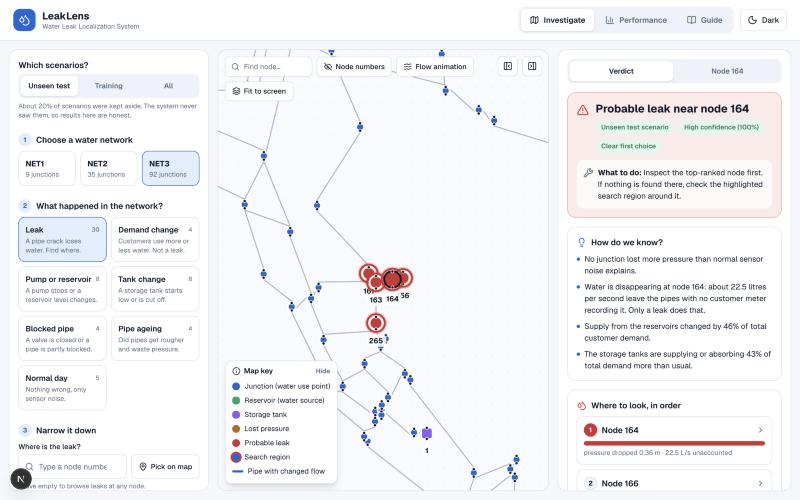
\includegraphics[width=0.93\linewidth]{figures/ui_light_leak.jpg}\caption{Investigate tab: left = choose, centre = map, right = verdict.}\end{figure}
\textbf{Header.} \emph{Investigate} (pick and analyse), \emph{Performance} (test results), \emph{Guide} (help and glossary), \emph{Light/Dark} theme (saved; first visit follows the computer).

\textbf{Left panel.}
\begin{itemize}
\item \textbf{Which scenarios?} \emph{Unseen test} (default, about 20\%, never seen in learning), \emph{Training} (the other 80\%), \emph{All}. Card counts change with this choice.
\item \textbf{1 Choose a water network:} NET1 / NET2 / NET3 with junction counts.
\item \textbf{2 What happened?} Seven cards (Leak, Demand change, Pump or reservoir, Tank change, Blocked pipe, Pipe ageing, Normal day); the small number is how many scenarios of that kind match the current filters.
\item \textbf{3 Narrow it down.} Leaks: \emph{Where?} (node number or \emph{Pick on map}; leave empty for any), \emph{How big?} (Tiny, Small, Medium, Large, Burst = 0.0001 to 0.01 m$^2$), \emph{Conditions} (Clean data, Noisy sensors, Hidden behind another event, Starts at another time). Other kinds: a word search. A counter shows matches; $\langle\ \rangle$ step through them; \emph{Surprise me} runs a random one. Each card shows an \textbf{Unseen test / Training} tag.
\item \textbf{Customers have smart demand meters:} ticked = per-node demand is used (normal). Unticked = the unaccounted flow ignores demand, so demand changes look like leaks.
\item \textbf{Analyse this scenario} runs the analysis.
\end{itemize}
\textbf{Map.} Circle = junction; green square = reservoir; purple square = tank; lines = pipes. After analysis: \textcolor{red!70!black}{red circle} = predicted leak (largest = first choice); orange = lost pressure (persistent drop above $\tau_P$, i.e.\ $d_i>1$); ring = \emph{search region}; blue pipe = mean flow change larger than 0.01 m$^3$/s. Tools: \emph{Find node}, \emph{Node numbers}, \emph{Flow animation}, \emph{Fit to screen}, panel hide buttons, \emph{Map key}.

\textbf{Right panel, Verdict tab.}
\begin{itemize}
\item \textbf{Verdict box:} for a leak ``Probable leak near node X'' (X = top node); otherwise the kind of event. Tags: \emph{Unseen test scenario} / \emph{Used in training} (with a warning that a right answer proves little), \emph{confidence} (High/Medium/Low from the top probability, with its \%), and for leaks \emph{Clear first choice} when (2nd score)/(1st score) $<0.5$, else \emph{Close call}. \emph{What to do} is a fixed sentence per kind.
\item \textbf{How do we know?} Fixed sentences, each shown when a number passes its limit:
\end{itemize}
\begin{center}\small\begin{tabularx}{\linewidth}{@{}p{5.2cm}Y@{}}\toprule
Sentence appears when & It says \\\midrule
\code{frac\_hit}$>0$ (else a ``none'' line) & share of junctions that lost more pressure than noise, and the biggest drop in m and its node (largest persistent drop, in metres $=d_{\max}\tau_P$) \\
\code{unacc\_ratio}$\ge1$ & water vanishes at node X: $a_X\times1000$ L/s unmetered \\
else \code{demand\_frac}$>0$ / else neither & metered demand explains the flow / all water accounted for \\
\code{pump\_drop}$>0.5$ & a pump lost that \% of flow \\
\code{source\_change}$>0.2$ / \code{tank\_change}$>0.2$ & reservoir supply / tank flow changed by that \% of total demand \\
\code{frac\_rise}$>0.05$ & some junctions gained pressure: blocked pipe or tank \\
\code{frac\_hit}$>0.5$ and \code{unacc\_ratio}$<1$ & loss spread over most of the network \\\bottomrule\end{tabularx}\end{center}
\begin{itemize}
\item \textbf{Where to look, in order:} top five nodes (leaks only). Bar = score relative to the first (at least 6\%). Text: ``pressure dropped X m'' (largest raw residual) and ``Y L/s unaccounted''. Click a node to open its tab. \emph{Search region} = first node + direct neighbours.
\item \textbf{Check against the answer key:} the true event; green/red badges: \emph{Cause correct?} and \emph{Top-1 hit} (or ``missed by $n$ pipe hops'').
\item \textbf{Technical details} (folded): probability for each kind; the 14 numbers in words; the formula \textbf{score $=A+0.3D$}; the network's $\tau_P$.
\end{itemize}
\textbf{Node tab.} \emph{Pressure now} = average over 24 h in the scenario; ``normal'' = average on the normal day; ``worst drop'' = largest raw residual; \emph{Unaccounted flow} in L/s; status \emph{Probable leak} / \emph{Lost pressure} / \emph{Looks normal}; chart of pressure by hour (normal blue, scenario red); the pipes touching the node.

\textbf{Performance tab.} Cards: leaks at exact node, real leak in first 5, false alarms, right cause (with training accuracy). Sections: finds leaks; small leaks; leak versus other causes (confusion matrix); unseen network; detailed numbers. All use test scenarios.

\textbf{Guide tab.} Five-step explanation, how to use the tab, kinds of situation, glossary, train/test explanation, limits. Words with a dotted underline show their definition on hover or tap.

\begin{figure}[H]\centering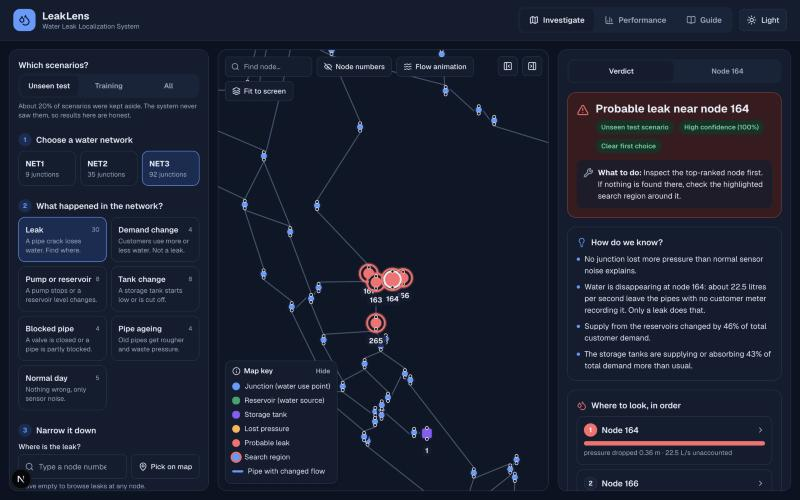
\includegraphics[width=0.93\linewidth]{figures/ui_dark_leak.jpg}\caption{Dark theme. Same screen, same numbers.}\end{figure}

%=========================================================
\section*{Part G: The software}\addcontentsline{toc}{section}{Part G: The software}
\begin{figure}[H]\centering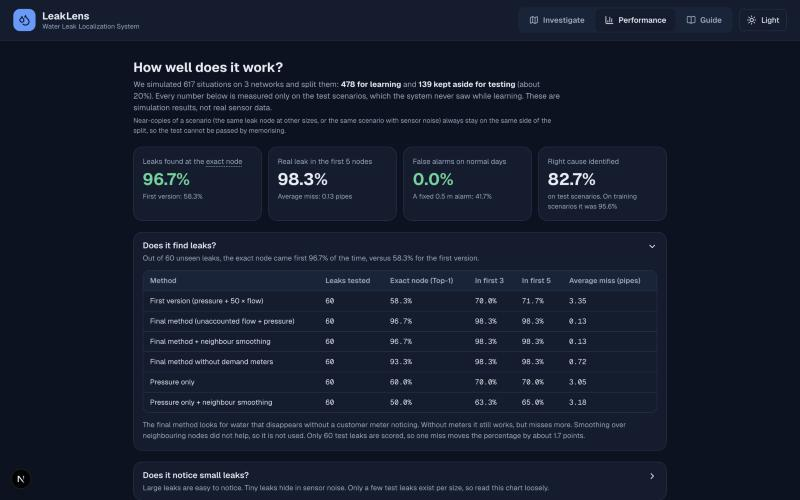
\includegraphics[width=0.93\linewidth]{figures/ui_performance.jpg}\caption{The Performance tab: it states the learning/testing split and reports test results only.}\end{figure}
\section{Code, data and how to run}
\textbf{Repository.} \code{simulation/} (build scenarios, run EPANET/WNTR); \code{ml\_pipeline/} (\code{dataset, features, detector, classifier, localizer, pipeline, split, train, evaluate}); \code{backend/} (FastAPI + SQLite); \code{frontend/} (Next.js dashboard); \code{data/} (networks, simulated scenarios, results); \code{reports/}.

\textbf{Backend.} At start-up it builds an SQLite table \code{scenarios} (id, network, name, group, event class, truth nodes, parameters, split tag) from the saved files.
\begin{center}\small\begin{tabularx}{\linewidth}{@{}>{\ttfamily}p{5.1cm}Y@{}}\toprule
Endpoint & Returns \\\midrule
GET /api/networks & networks, junction and scenario counts \\
GET /api/scenarios?network= & scenario list with parameters and the split tag \\
GET /api/network?network= & node positions and pipes (for the map) \\
GET /api/analyze/\{id\}?use\_demand\_meters= & verdict, probabilities, 14 numbers, ranked nodes, search region, affected nodes, per-node and per-pipe numbers, split tag, answer key \\
GET /api/evaluation & the saved test results \\\bottomrule\end{tabularx}\end{center}
\textbf{Run order.}
\begin{enumerate}
\item \code{python simulation/build\_scenarios.py} \quad (scenario list)
\item \code{python simulation/generate\_dataset.py --force} \quad (simulate, about 30 s)
\item \code{python ml\_pipeline/train.py} \quad (fit on training scenarios, writes \code{split.json})
\item \code{python ml\_pipeline/evaluate.py} \quad (scores on test scenarios)
\item \code{cd backend \&\& uvicorn main:app --port 8000}
\item \code{cd frontend \&\& npm run dev} \quad (open \code{http://localhost:3000})
\end{enumerate}

\section{Questions the team may be asked}
\begin{itemize}
\item \textbf{Why does it work?} Because water must balance at every node; unmetered loss at one node can only be a leak.
\item \textbf{Why 80/20, and why grouped?} Testing on learned scenarios proves nothing; near-copies (same leak node at other sizes, noisy twins) would make the test too easy.
\item \textbf{Why is test accuracy (82.7\%) below training (95.6\%)?} The forest partly memorises its 478 rows; the ranking formula is not trained, so its Top-1 barely changes (96.7\% vs 97.8\%).
\item \textbf{Why 0\% false alarms?} The threshold is learned from the network's own noise; but there are only 12 normal test days, so the true rate is not exactly zero.
\item \textbf{Why is weight 0.3 used?} Chosen during development to let pressure break ties when flow data are weak. It was not re-tuned after the split.
\item \textbf{What if there are no demand meters?} Demand changes look like small leaks; Top-1 falls to 93.3\% and cause accuracy to 74.1\%.
\item \textbf{Does it work on a real network?} Unknown. Everything is simulated.
\end{itemize}

\section{Honest limitations}
Simulation only; small test set and a single split; ranking settings chosen before the split; per-node demand meters assumed; leaks inside sensor noise are called normal; the biggest leaks are hardest to pinpoint; pump, tank, blockage and ageing are confused with each other and do not transfer to unseen networks; Net3 nodes 61 and 601 and hour 21 are ignored; pump speed changes were not simulated (the simulator does not support them).

\section{Next steps (Semester 2)}
Missing and sparse sensors with graph-based sensor placement; estimating demand where nodal meters do not exist; several simultaneous leaks; cause models that transfer across networks (including graph or algorithm-informed models compared with this interpretable baseline); repeated re-splitting for tighter error bars; real or public benchmark data.

\section{Glossary}
\begin{center}\small\begin{tabularx}{\linewidth}{@{}>{\bfseries}p{2.7cm}Y@{}}\toprule
Baseline & the simulated normal day used as reference \\
Scenario & one 24-hour simulation with a known true answer \\
Junction / reservoir / tank / pump & water use point / source / storage / machine adding pressure \\
Pressure (m) & push of the water, as metres of water column \\
Flow (L/s) & litres passing a point each second \\
Demand, demand meter & water customers draw; meter that reports it \\
Unaccounted flow & water leaving a node with no meter behind it = leak flow \\
Noise unit & measured value divided by the learned noise limit; 1 = at the limit \\
Persistence & a change counts only if it lasts two hours in a row \\
$\tau_P$ & learned pressure noise threshold ($\max\{0.1,4\sigma_P\}$) \\
Quiet check & all signals within noise $\Rightarrow$ normal day \\
Random forest & 300 small decision trees that vote on the kind of event \\
Confidence & the top probability from the forest (High $\ge85\%$, Medium $\ge60\%$) \\
Train / test & scenarios learned from (about 80\%) / kept aside (about 20\%) \\
Precision, recall, $F_1$ & how often an alarm is real; how many real events are caught; their balance \\
False-alarm rate & share of normal days wrongly flagged \\
Accuracy, macro-$F_1$ & share correct; average $F_1$ over kinds \\
Confusion matrix & table of true kind versus system answer \\
Top-1 / Top-5 & true leak is first / within first five \\
Hop / metres & pipes (or pipe length) between guess and truth \\
Search region & top node plus its direct neighbours \\
Leave-one-network-out & train on two networks, test on the third \\\bottomrule\end{tabularx}\end{center}

\newpage
\section*{Appendix A: formula cheat sheet}\addcontentsline{toc}{section}{Appendix A: formula cheat sheet}
\begin{center}\small\begin{tabularx}{\linewidth}{@{}>{\bfseries}p{3.3cm}Y@{}}\toprule
Quantity & Formula \\\midrule
Leak flow & $Q_\ell=0.75\,A\sqrt{2gP}$ \\
Customer demand & $D_i(t)=D_{\text{base},i}\,m(t)\,f$ \\
Head loss (ageing) & $h_f=10.67\,L\,Q^{1.852}/(C^{1.852}d^{4.87})$ \\
Residual & $r_i(t)=P^0_i(t)-P^1_i(t)$ \\
Persistent peak & $\max_t\min\{x(t),x(t{+}1)\}$ \\
Pressure noise threshold & $\tau_P=\max\{0.1,\,4\sigma_P\}$ \\
Drop / rise (noise units) & $d_i=\max\{0,\text{peak}(r_i)\}/\tau_P$;\ $g_i=\max\{0,\text{peak}(-r_i)\}/\tau_P$ \\
Net inflow & $\text{div}_i(t)=\sum_p\operatorname{sign}(p,i)Q_p(t)$ \\
Unaccounted flow & $a_i(t)=\Delta\text{div}_i(t)-\Delta D_i(t)$;\ in noise units $a_i=\max\{0,\text{peak}(a_i)\}/(4\sigma_{a,i})$ \\
Quiet check & $d_{\max}<1,\ g_{\max}<1,\ a_{\max}<1,\ \text{flow\_frac}<0.1,\ \text{demand\_frac}=0\Rightarrow$ normal \\
Confidence label & top probability $\ge0.85$ High, $\ge0.60$ Medium, else Low \\
Leak score & $\text{score}_i=a_i/\max a+0.3\,d_i/\max d$ \\
Clear first choice & $\text{score}_2/\text{score}_1<0.5$ \\
Precision / recall & $TP/(TP+FP)$;\ $TP/(TP+FN)$ \\
$F_1$ & $2PR/(P+R)$ \\
False-alarm rate & $FP/(FP+TN)$ \\
Accuracy & (correct)/(all) $=115/139$ \\
Macro-$F_1$ & mean of the seven per-kind $F_1$ \\
Top-$k$ & $\frac1N\sum_s\mathbf 1[r_s\le k]$ \\
Mean hops & $\frac1N\sum_s\text{hops}(\hat n_s,n_s)$ \\
Split & about 80\% train / 20\% test, grouped, seed 42 \\\bottomrule\end{tabularx}\end{center}

\section*{Appendix B: code map}\addcontentsline{toc}{section}{Appendix B: code map}
\begin{center}\small\begin{tabularx}{\linewidth}{@{}>{\ttfamily}p{4.3cm}Y@{}}\toprule
File & What it does \\\midrule
simulation/simulator.py & runs one scenario in WNTR; events: leak, demand, hydrant, pump outage, reservoir head, tank level, closed or throttled pipe, roughness, combined; adds sensor noise \\
simulation/build\_scenarios.py & builds the scenario list from each network's own layout; checks blockages converge \\
simulation/generate\_dataset.py & simulates all scenarios, saves pressure, flow and demand CSVs, finds ignored nodes and hours \\
ml\_pipeline/dataset.py & loads data and the pipe graph; incidence matrix; hops and metres \\
ml\_pipeline/split.py & the grouped 80/20 split (seed 42) \\
ml\_pipeline/features.py & noise learning, unaccounted flow, the 14 numbers, quiet check \\
ml\_pipeline/detector.py & persistence rule and the learned pressure threshold \\
ml\_pipeline/classifier.py & random forest and decision tree definitions, class names \\
ml\_pipeline/localizer.py & leak score and ranking (and the first-version formula for comparison) \\
ml\_pipeline/pipeline.py & one function that analyses a scenario end to end (used by the API and the evaluation) \\
ml\_pipeline/train.py & fits the models on training scenarios only \\
ml\_pipeline/evaluate.py & scores everything on test scenarios and writes the result files \\
backend/main.py, catalog.py & server start-up; builds the SQLite scenario table \\
backend/routers/ & the API endpoints \\
frontend/src/app/page.tsx & dashboard layout and logic \\
frontend/src/components/ & ScenarioPicker, NetworkMap, ResultView, PerformanceView, GuideView, Term, ThemeToggle \\
data/results/ & \code{evaluation\_summary.json}, \code{split.json}, \code{features.csv}, \code{decision\_rules.txt}, per-scenario results \\\bottomrule\end{tabularx}\end{center}
\end{document}
